\documentclass[addpoints]{exam}

\usepackage{comment}
\usepackage{graphbox}
\usepackage{hyperref}
\usepackage{listings}
\usepackage{subcaption}
\usepackage{tabularx}
\usepackage{tikz}
\usetikzlibrary{positioning}

% Header and footer.
\pagestyle{headandfoot}
\runningheadrule
\runningfootrule
\runningheader{CS 440}{HW 2: Interactive WebGL}{Fall 2023}
\runningfooter{}{Page \thepage\ of \numpages}{}
\firstpageheader{}{}{}

\qformat{{\large\bf \thequestion. \thequestiontitle}\hfill[\totalpoints\ points]}
% \qformat{{\large\bf \thequestion. \thequestiontitle}\hfill}
\boxedpoints

\graphicspath{{images/}}

\title{Homework 2: Rendering with WebGL}
\author{CS 440 Computer Graphics\\Habib University}
\date{Fall 2023}

\begin{document}
\maketitle

Each problem below specifies the names of the files that you have to submit for it. Please make sure that your submitted files have the indicated names. Any files in your GitHub repository with these names at the time of the deadline will be considered your submission. A required file with a \texttt{.glsl} extension may be replaced with a file of the same name with a \texttt{.c} extension. Some of the problems refer to the {\tt map\_point} function from the previous homework.

We will use the utility files from \href{https://bit.ly/3Bqt8XG}{the website} of the newer edition of the textbook. Specifically, we will make use of the files containing ``ES6" in their names. These supersede similarly named files in the folder in that they are compliant with recent JavaScript (JS) standards which deprecate older features that are, in some cases, now considered insecure. In your HTML files, you may include the files, \texttt{MVES6.js} and \texttt{initShadersES6.js}, over the web, or you may include local copies.

\begin{comment}
  \begin{itemize}
  \item Make colorabrs in different ways. Explain we will do it in many ways before ultimately doing it the right way.
    \begin{itemize}
    \item pass canvas width, W, as a uniform
    \item draw W vertical lines. (2W vertices) assign colors in verex shader, with menu choice for grayscale or colors
    \item make 2 triangles, do not send color, rather compute color for each fragment in fragment shader based on fragCoord
    \item make 2 triangles, assign color to vertices
    \item use above approach to render the colorbar with 6 or fewer vertices,
    \item [stretch] Draw both bars together using the above technique, either in different viewports in the same canvas, or on different canva on the same page.
    \end{itemize}
  \end{itemize}
\end{comment}

\begin{questions}

\titledquestion{Essentials}
  \label{q:bars}
  \begin{parts}
  \part Go over \href{https://webgl2fundamentals.org/webgl/lessons/webgl-shaders-and-glsl.html#uniforms}{this page} for a quick recap on WebGL2 Shaders and GLSL. On the page, you may skip the sections titled, ``Textures in Vertex Shaders'', and, ``Textures in Fragment Shaders''.
  \part Go over the page ``Including shaders from external files'' under the \texttt{HW 2} module on Canvas. Make sure to understand and follow the instructions. All the problems in this homework will follow the format described on the page.
  \end{parts}

\titledquestion{Color Interpolation}
  \label{q:colorbar}.
  
  \vspace{-30pt}
  \begin{center}
    \includegraphics[width=\linewidth]{barbw}\\
    \vspace{-75pt}\includegraphics[width=\linewidth]{barrgb}
  \end{center}
  \vspace{-50pt}
  Recall the colorbars from the previous homework. We will draw them using different methods in order to illustrate various WebGL functionality. For each part below, your render should occupy the entirety of the \texttt{canvas} (you may draw a border around the canvas to highlight its boundary), the \texttt{canvas} should be adequately sized, and your rendered colorbar should appear smooth as shown above.
  \begin{parts}
  \part[5]\label{p:lines} Draw the grayscale colorbar by drawing a colored vertical line for each column in the \texttt{canvas}. In your JS file, compute and assign colors to the endpoints of the lines. Use your \texttt{map\_point} function from the previous homework to compute vertex coordinates and colors across the canvas.  \\
    \underline{Tip}: It will be helpful to define the \texttt{start} and \texttt{end} values to iterate over the canvas. Use these for iteration and for \texttt{map\_point}.\\
    \underline{Note}: If your colorbar renders with some vertical bands of the background color, adjust the \texttt{start} and \texttt{end} limits until the bands disappear.\\
  \underline{Files}: 2a.html, 2a.js, 2a-vshader.glsl, 2a-fshader.glsl
\part[5]\label{p:fcoord} The above method is tedious. In order to compute a number of lines in the order of the width of the canvas, you have to compute and transfer twice as many vertices and colors. In this part, we will draw the same colorbar by drawing two triangles using \texttt{gl.TRIANGLE\_STRIP}. Define 4 vertices with appropriate coordinates. Assign color in the fragment shader to each fragment based on its \texttt{gl\_FragCoord} and the canvas width. \texttt{gl\_FragCoord.xy} are the fragment's 2D coordinates in the canvas. Here, you only require \texttt{gl\_FragCoord.x}. You also need to prove the canvas width to your fragment shader. Do so by sending it from your JS program as a \texttt{uniform} value.\\
  \underline{Files}: 2b.html, 2b.js, 2b-vshader.glsl, 2b-fshader.glsl
\part[5] The approach in part \ref{p:fcoord} is arguably more intensive than the one in part \ref{p:lines}. You have to assign color to many more fragments in part \ref{p:fcoord} than vertices in part \ref{p:lines}. But there are several advantages.
  \begin{itemize}
  \item Unlike the vertices which you computed in \ref{p:lines}, the fragments are automatically computed by the pipeline.
  \item You have to write much less code to assign color to the fragments.
  \item The fragment shaders execute in parallel on the GPU whereas the JS code executes serially on the CPU.
  \end{itemize}
  Generally, we want to offload as much work to the pipeline as possible. In this part, we send the same 4 vertices to the GPU and their colors. With this approach, we do not even have to compute the color in the fragment shader. The pipeline computes the color for us. This is the best approach!\\
  \underline{Files}: 2c.html, 2c.js, 2c-vshader.glsl, 2c-fshader.glsl
\part[5] Using the same approach as the previous part, draw the RGB colorbar using 6 vertices and \texttt{gl.TRIANGLE\_FAN}.\\
  \underline{Files}: 2d.html, 2d.js, 2d-vshader.glsl, 2d-fshader.glsl
  \end{parts}


\titledquestion{The Mandelbrot Set}

  The sequence $z_n$ for a complex number, $c$, is defined for $n\geq 0$ as
  \[
    z_n(c) = \left\{
      \begin{array}{l@{\quad}l}
        0 & n = 0\\
        z^2_{n-1}(c)+c & \textrm{otherwise}
      \end{array}
    \right.
  \]

  \begin{figure}
    \centering
    \begin{tabular}{cc}
      \includegraphics[width=.47\linewidth]{mandelbrot1}& \includegraphics[width=.47\linewidth]{mandelbrot2}\\
      (a) & (b)
    \end{tabular}
    \caption{The Mandelbrot set up to $n_t = 100$. The points at the corners of the windows are outside the circle of radius 2, and $z_n$ escapes for these points at $n=1$. They are completely red. The points in blue toward the center of the image are the ones for which $z_n$ has not yet escaped. (a) Uniform color interpolation from Red to Green to Blue. (b) Adjusted color interpolation on the same data.}
    \label{fig:mandelbrot}
  \end{figure}
  
  The \href{http://en.wikipedia.org/wiki/Mandelbrot_set}{Mandelbrot set}, $M$, is the set of all complex numbers, $c$, for which $z_n(c)$ is \textit{bounded}, i.e. $|z_n|$ is finite for all $n$. It can be shown for a given $c$ that if $|z_{n}(c)| > 2$ for some $n = n_0$, then the sequence $z_n(c)$ {\it escapes to infinity}, i.e. $z_n(c)$ is not bounded for $n > n_0$. Thus, for $c\in M$, $|z_n(c)| \leq 2$ for all $n\geq 0$. Since $z_1(c) = c$, we also have that $|c| \leq 2$. Therefore, $c\in M$ implies that:
  \begin{enumerate}
  \item $|c|\leq 2$
  \item $\forall n\geq 0:\, |z_n(c)|\leq 2$
  \end{enumerate}
  Condition 1 implies that every $c\in M$ lies within the circle in the complex plane centered at the origin and with radius 2. The value of $n$ for which condition 2 becomes false for a given $c$ is dubbed the {\it escape time} of $c$.

  \underline{Example}: Consider the complex numbers and their corresponding sequences up to $z_5$ in Table \ref{tab:mandelbrot}.
  \begin{table}
  \[
    \begin{array}{c|*{4}{|c}}
      & c=(3+4j) & c=(1+1j) & c=(0.5+0.5j) & c=(-0.5-0.5j)\\\hline\hline
      z_0(c) & 0 & 0 & 0 & 0\\
      |z_0(c)| & 0 & 0 & 0 & 0\\\hline
      z_1(c) & (3+4j) & (1+1j) & (0.5+0.5j) & (-0.5-0.5j)\\
      |z_1(c)| & 5.0 & 1.41 & 0.71 & 0.71\\\hline
      z_2(c) &  & (1+3j) & (0.5+1j) & (-0.5+0j)\\
      |z_2(c)| &  & 3.16 & 1.12 & 0.5\\\hline
      z_3(c) &  &  & (-0.25+1.5j) & (-0.25-0.5j)\\
      |z_3(c)| &  &  & 1.52 & 0.56\\\hline
      z_4(c) &  &  & (-1.69-0.25j) & (-0.69-0.25j)\\
      |z_4(c)| &  &  & 1.71 & 0.73\\\hline
      z_5(c) &  &  & (3.29+1.34j) & (-0.09-0.16j)\\
      |z_5(c)| &  &  & 3.55 & 0.18\\\hline
    \end{array}
  \]
  \caption{Examples of $z(n), 0\leq n\leq 5$ for some values of $c$. The magnitude of each value of $z(n)$ is shown until it escapes.}
  \label{tab:mandelbrot}
\end{table}
\begin{itemize}
  \item We see that $z_1=c$. This follows from the definition of $z_n$.
  \item For the first number, $(3+4j)$, we see that $|z_1|>2$. We can therefore say that $z_n$ will escape to infinity and the escape time of $(3+4j)$ is 1. This is expected as $(3+4j)$ lies outside the circle at the origin with radius 2.
  \item The second number, $(1+1j)$, lies within the required circle. But it escapes at n=2.
  \item The escape time for the third number, which is also inside the circle, is 5.
  \item The fourth number is also inside the circle and has not escaped until n=5. It may escape later or it may not. We cannot say.
  \end{itemize}
  
  We want to render the Mandelbrot set up to a certain value of $n=n_t$. We map to our viewport, the portion of the complex plane in which the ranges of the real and imaginary axes are $[-2,2]$ and $[-2j,2j]$ respectively. Thus, each pixel in the viewport maps to a complex number. We will color each pixel according to the escape time of its corresponding complex number. In Figure \ref{fig:mandelbrot}, complex numbers that escape early are assigned red and those that have not escaped till $n=n_t$ are assigned blue. Complex numbers with intermediate escape values are assigned interpolated colors.

  Various steps are involved.
  \begin{enumerate}
  \item Map the x extent of the viewport to $[-2,2]$ on the real axis in the complex plane.
  \item Map the y extent of the viewport to $[-2j,2j]$ on the imaginary axis in the complex plane.
  \item Find the escape time of the complex number corresponding to each pixel in the viewport.
  \item Compute a color for a given escape time.
  \end{enumerate}

  \begin{parts}
  \part[10] Visualize the Mandelbrot set by assigning colors in the fragment shader, similar to Q\ref{q:bars}\ref{p:fcoord}). You may specify a value for $n_t$, e.g., $20$ in the vertex shader.\\
    \underline{Tips}:
    \begin{itemize}
    \item Write and use relevant functions in the fragment shader file to perform arithmetic on complex numbers.
    \item Write and use a version of the \texttt{map\_point} function in the fragment shader file.
    \item Use \texttt{uniform} to pass the \texttt{canvas} dimensions to the fragment shader.
    \item You will find that a simple linear interpolation between the colors for $n=1$ and $n=n_t$ will lead to a bland visualization as seen in Figure \ref{fig:mandelbrot}a). Implement a more discriminating color scheme for the escape times. You may implement any coloring scheme that sufficiently distinguishes between different escape times.
    \end{itemize}
    
  \part[10] Include a mechanism on your page, e.g. a slider, to control the value of $n_t$ within a reasonable range. The render should update in response to changes in the value.\\
  \end{parts}
  \underline{Files}: mandelbrot.html, mandelbrot.js, mandelbrot-vshader.glsl, mandelbrot-fshader.glsl

  \titledquestion{Boundary and Interior}[10]

    \underline{Problem}: We are going to render a triangle along with its boundary edges. The triangle and its edges are colored independently.
    
    \underline{Task}: Render the (filled) triangle and its boundary as described above and include in your page, interactive controls for the following.
  \begin{itemize}
  \item Set the RGB colors of each of the boundary vertices.
  \item Set the RGB colors of each of the triangle (interior) vertices.
  \item Toggle the display of the boundary.
  \item Toggle the display of the triangle (the interior).
  \item Assign random colors to all of the boundary vertices.
  \item Assign random colors to all of the triangle vertices.
  \end{itemize}
  \underline{Files}: colors.html, colors.js, colors-vshader.glsl, colors-fshader.glsl
  
  \titledquestion{Subdivision: $\lim\limits_{n\rightarrow\infty} \diamond = \circ$}
  \begin{center}
    \includegraphics[width=\linewidth]{circle}
  \end{center}

  \begin{tabularx}{\linewidth}{lX}

    \raisebox{-\totalheight}{
      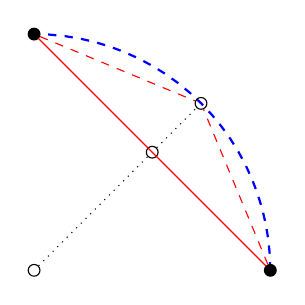
\begin{tikzpicture}
        \draw [blue,thick,dashed,domain=0:90] plot ({3*cos(\x)}, {3*sin(\x)});    
        node[circle,fill]{}(
        \node [draw,circle,fill,inner sep=1.5pt] at (0,3) (a){};
        \node [draw,circle,fill,inner sep=1.5pt] at (3,0) (b){};
        \node [draw,circle,inner sep=1.5pt] at (0,0) (c){};
        \node [draw,circle,inner sep=1.5pt] at (1.5,1.5) (p){};
        \node [draw,circle,inner sep=1.5pt] at (2.12,2.12) (q){};

        \draw [red] (a) -- (b);
        \draw [dotted] (c) -- (p);
        \draw [dotted] (p) -- (q);
        \draw [red, dashed] (a) -- (q);
        \draw [red, dashed] (b) -- (q);
      \end{tikzpicture}
    }
    &
      \underline{Problem}: For rendering purposes, a computer approximates a smooth shape with a many-sided polygon. We will approximate a circle with a successively refined diamond shape shown on the left in the figure above. Each successive shape in the figure is a refinement or \textit{subdivision} of the previous shape. The subdivision step inserts edge midpoints into the shape and projects them to the circumference of the circle being approximated. This is illustrated in the figure on the left. The red solid line approximates the blue arc. In the subdivision step, the midpoint of the solid line is inserted and projected to the arc. The red solid line is then replaced with the red dashed lines.
  \end{tabularx}

    \underline{Task}:
    \begin{parts}
    \part[5] Render the level 0 circle (0 subdivisions). This is the diamond shown above.
    \part[10] Include a mechanism to interactively increase or decrease the number of subdivision steps. The render should update interactively according to the change in recursion level.
    \end{parts}
    \underline{Files}: circle.html, circle.js, circle-vshader.glsl, circle-fshader.glsl
  
  \titledquestion{Koch Snowflake}

\begin{tabularx}{1.0\linewidth}{cX}
    \includegraphics[width=.3\textwidth,align=t]{koch1}
  &
    \vspace{10pt} \underline{Problem}: We will render a \href{https://en.wikipedia.org/wiki/Koch_snowflake}{Koch snowflake} which is a \href{http://mathworld.wolfram.com/Fractal.html}{fractal} generated by repeatedly applying a fixed transformation to all line segments. The figure on the left shows the starting shape on the top left and, proceeding clockwise, the results of successive applications of the transformation which is illustrated below.
    
    {\begin{tabularx}{0.63\textwidth}{cX}
    \includegraphics[scale=.7,align=t]{koch2}
      & The line segment $AB$ is replaced by the polyline $APQRB$ where the length of all shown line segments is equal to $\frac{|AB|}{3}$.
    \end{tabularx}}
\end{tabularx}

\underline{Task}:
\begin{parts}
    \part[5] Render the level 0 snowflake (0 recursive steps). This is the triangle shown above.
    \part[10] Include a mechanism to interactively increase or decrease the number of recursive steps applied to the Level 0 shape. The render should update interactively according to the change in recursion level.
\end{parts}
    \underline{Files}: koch.html, koch.js, koch-vshader.glsl, koch-fshader.glsl
  
  \titledquestion{Sierpinski Triangle}
  
  \begin{figure}
    \centering
    \begin{tabular}{cc}
      \includegraphics[width=.4\linewidth]{sierpinski}
      &
      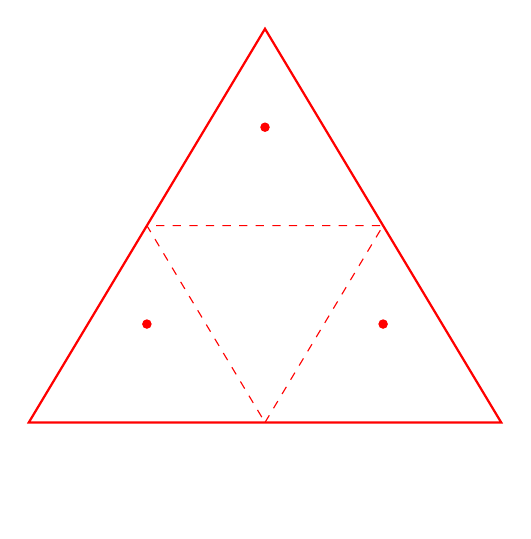
\begin{tikzpicture}
        \draw[red,thick] (0,0) -- (6,0) -- (3,5) -- cycle;
        \draw[red,dashed] (3,0) -- (4.5,2.5) -- (1.5,2.5) -- cycle;
        \draw[red,fill] (1.5, 1.25) circle (1.5pt);
        \draw[red,fill] (4.5, 1.25) circle (1.5pt);
        \draw[red,fill] (3, 3.75) circle (1.5pt);
        
        \node at (3,-1) {};
      \end{tikzpicture}\\
      (a) & (b)
    \end{tabular}
    \caption{(a) A Sierpinski triangle at recursion level 5. (b) The triangles that are subdivided in the recursive step in the generation of the Sierpinski triangle.}
    \label{fig:sierpinski}
  \end{figure}
  
\underline{Problem}: We will render the \href{https://en.wikipedia.org/wiki/Sierpinski_triangle}{Sierpinski triangle}, a \href{https://en.wikipedia.org/wiki/Self-similarity}{self-similar} geometric shape with many interesting properties, not the least of which is the variety of ways in which it can be generated. A sample Sierpinski triangle is shown in Figure \ref{fig:sierpinski}a).

We will generate the Sierpinski triangle recursively as illustrated in Figure \ref{fig:sierpinski}b). Starting with a triangle, connect all its edge midpoints. This yields 4 new triangles. Repeat the process for all the new triangles shown with a dot in them. Do not subdivide the triangle in the middle (without a dot). Note that the dots in the figure are for demonstration purposes only--they are not part of the Sierpinski triangle.

\underline{Task}:
\begin{parts}
\part[5] Render the level 0 Sierpinski triangle (0 recursive steps). This is just a triangle.
\part[10] Include a mechanism to interactively increase or decrease the number of recursive steps applied to the Level 0 shape. The render should update interactively according to the change in recursion level.
\end{parts}
  \underline{Files}: sierpinski.html, sierpinski.js, sierpinski-vshader.glsl, sierpinski-fshader.glsl


\titledquestion{Polygons Galore}
  \label{q:galore}
  
  \begin{tabularx}{\linewidth}{lX}
    \includegraphics[width=.3\textwidth,align=t]{galore}
    &
      \vspace{20pt} \underline{Task}: We love polygons and cannot get enough of them. We will draw a limited set of polygons whose vertices are specified by the user through mouse clicks and are connected as per the current \textit{drawing mode}. For example, if \textit{triangle mode} is on, every 3 successive vertices will be connected to form a triangle.
  \end{tabularx}

  \underline{Task}: 
  \begin{parts}
  \part[5] Interactively draw triangles and quadrilaterals based on vertices specified by mouse clicks in the canvas. Your program should support two drawing modes--triangle mode (default) and quad mode. Vertices that are not yet part of a polygon are drawn as points.
  \part[5] Pressing \texttt{r} or \texttt{R} resets to default. That is, the canvas is cleared and the drawing mode is set to triangle mode.
  \part[10] Pressing \texttt{t} or \texttt{T} toggles between the drawing modes. Vertices that have not yet completed a polygon at the time of the toggle should be handled according to the new mode, they should not be discarded. Polygons drawn before the toggle should not be affected.
  \end{parts}
  \underline{Files}: galore.html, galore.js, galore-vshader.glsl, galore-fshader.glsl

\end{questions}

\end{document}

%%% Local Variables:
%%% mode: latex
%%% TeX-master: t
%%% End:


Thanks, Asif, for the invitation. Adam's classmate, Zoha, is the wrong gender for this :) The brother, Musa, is 2 years younger so is hesitant to join as he will not know the people. Both of them are anyway into football and have classes 3 days a week including Saturday. Also, we are not as early risers as you :) My wife, Mifrah, tells that your family always gets stuff done early int he day. Unfortunately, our family is full of late rising sleepyheads! So, if start a football league which meets slightly later in the day, we will be very happy to join. Again, thank you very much for the invitation. I hope Adam has a lot of fun!